% !TEX root = ../../thesis.tex
\chapter{Theory}
\section{Superconductors}
The most well known property of superconductors are their perfect conductivity\footnote{Discovered by H.K. Onnes in 1911.} and their perfect diamagnetism\footnote{Discovered by W. Meissner and R. Ochsenfeld in 1933.}. A microscopic description of the effect is given by Bardeen, Cooper and Schieffer (BCS theory) and phenomenologically by the Ginzburg-Landau theory.\cite{tinkhamIntroductionSuperconductivity} This section will highlight the relevant parts of these theories for our research.

BCS theory shows that superconductivity, on the atomic scale, is a result of the creation of paired electrons. We call these Cooper pairs. The Cooper pairs form from an phonon-mediated attractive interaction that overcomes the Coulomb repulsion between two electrons.\cite{bardeenTheorySuperconductivity1957} Electrons have half-integer spin, which means a Cooper pair, consisting of two electrons, has integer spin. As such Cooper pairs are bosons.

Bosons, contrary to fermions, can occupy the same quantum state. At low temperatures bosons form a condensate. All Cooper pairs in the condensate occupy the same macroscopic wavefunction\footnote{This is by definition of a `condensate' the case.}.
\begin{equation}
	\Psi = \left|\Psi\right| \exp(i\varphi)
	\label{eqn:GL-wavefunction}
\end{equation}
Both $\left|\Psi\right|$ and $\varphi$ are functions of position. The behaviour of this wave function is described by the Ginzburg-Landau theory. In this theory we can view $|\Psi|^2$ as the density of Cooper pairs (units of \unit{\per\cubic\meter}). The super current density (\unit{\ampere\per\square\meter}) is given by\footnote{See \citetitle{tinkhamIntroductionSuperconductivity} equation 4.14a.}:
\begin{equation}
	\vec{J_s} = e^* |\psi|^2 \vec{v_s} = \frac{e^*}{m^*} |\psi|^2 \left(\hbar \nabla \varphi-\frac{e^*}{c} \vec{A}\right) \stackrel{\text{SI}}{=} \frac{e}{m_e} |\psi|^2 \left(\hbar \nabla \varphi + 2e \vec{A}\right)
	\label{eqn:super-current}
\end{equation}

\subsection{Characteristic length scales}
\label{sec:characteristic-length-scales}
There are two important length scales for superconductors. We will focus on these length scales mainly in relation to the Ginzburg-Landau theory. See Figure \ref{fig:characteristic-lengths} for a schematic depiction.

\begin{figure}[ht!]
	\centering
	\def\svgwidth{\textwidth}
	\import{figures}{characterstic_lengths.pdf_tex}
	\caption{Schematic depiction of the characteristic lengths $\xi$ and $\lambda$. The Cooper-pair density $|\Psi(x)|^2$, also referred to as $n_s$, falls off on a scale $\xi$. The magnetic field gets shielded by the superconductor using a shielding current and falls off on a scale $\lambda$. The S and N denote the `superconducting' and `normal' regimes respectively.}
	\label{fig:characteristic-lengths}
\end{figure}

The first is the scale over which the Cooper-pair density $|\Psi|^2$ can change. This is the so called coherence length, $\xi(T)$. $\xi$ decreases when the temperature increases.\cite{tinkhamIntroductionSuperconductivity}

The second length scale is the penetration depth $\lambda$. It is a measure for the `stiffness' of the phase. A small $\lambda$ means $\varphi$ can change easily. This means larger super currents are possible. The currents can screen magnetic fields which penetrate roughly on the same length scale. The penetration depth in Ginzburg-Landau theory at \qty{0}{\kelvin} is given by\footnote{See \citetitle{tinkhamIntroductionSuperconductivity} equation 4.8.}:
\begin{align}
	\lambda(0) &= \sqrt{\frac{m^*c^2}{4\pi|\psi|^2e^{*2}}} \stackrel{\text{SI}}{=} \sqrt{\frac{m_e}{2|\psi|^2e^2\mu_0}}
	\label{eqn:london-penetration-depth}
\end{align}
The penetration depth too is dependent on temperature and decreases for higher temperatures. For more information on length scales the reader is referred to \citetitle{tinkhamIntroductionSuperconductivity} by \citeauthor{tinkhamIntroductionSuperconductivity}.

\section{Josephson effect}
\label{sec:josephson-effect}
When two superconductors are separated by a weak link\footnote{This can be an insulator, normal metal, different superconductor or a constriction.} a supercurrent can flow between them. Josephson showed in 1962 that for two superconductors separated by an insulating tunnelling barrier the current is given by\cite{tinkhamIntroductionSuperconductivity}:
\begin{equation}
	I_s = I_c \sin(\Delta \varphi)
	\label{eqn:1st-josephson-relation}
\end{equation}
Where $\Delta \varphi$ is the difference in phase between the two condensates as described by Ginzburg-Landau theory, see Eq. \ref{eqn:GL-wavefunction}. Furthermore $I_c$ is the critical current which is a junction property. This equation is generally known as the first Josephson equation. The relation between $I_s$ and the phase difference is the current-phase relation. In general this does not have to be purely sinusoidal.\cite{golubovCurrentphaseRelationJosephson2004a}

In the more general case we first define the gauge invariant phase\footnote{See \citetitle{tinkhamIntroductionSuperconductivity} equation 6.11. The equation is valid in both Gaussian and SI units.}:
\begin{equation}
	\gamma = \Delta \varphi - \frac{2\pi}{\Phi_0}\int \vec{A} \cdot d\vec{l}
	\label{eqn:gauge-invariant-phase}
\end{equation}
We are required to do so as $\Delta \varphi$ is not uniquely determined for a given physical situation whilst $I_s$ is.\cite{tinkhamIntroductionSuperconductivity} It simply transforms $I_c \sin(\Delta \varphi) \to I_c \sin(\gamma)$. To now generalize our current-phase relation we write:
\begin{equation}
	I_s = I_c f(\gamma)
\end{equation}
Here we have defined $f(\gamma)$ which is the current-phase relation. In general it has the following properties\cite{golubovCurrentphaseRelationJosephson2004a}:
\begin{equation}
	f(\gamma) = f(\gamma + 2\pi) \quad f(\gamma) = -f(-\gamma) \quad f(2\pi n) = f(\pi m) = 0
\end{equation}
With $m,n \in \mathcal{N}$. The last statement is not always true. There have been reports of $4\pi$ periodic CPRs.\cite{endresCurrentPhaseRelation2023}

\section{dc-SQUID magnetometers}
% 1. Reiterate that junctions are described by a CPR
% 2. Note that CPRs have no currents above Ic!
% 3. Explain that above Ic, junctions operate in the dynamic regime. You could use the second Josephson relation, or the RCSJ model, or just cite something.
% 4. Now when two junctions are operated in parallel, the dynamic regime starts at I=2Ic.
% 5. Then explain that in superconductors J \propto A and \propto \nabla \phi so that magnetic vector potential and phi are coupled: we can tune the phase in this loop by applying a flux!
% 6. Then cite the interference pattern: Imax = 2Ic|cos(2piPhi/Phi0)|.
% 7. Then start a new subsection that explains how to read out a SQUID
% A dc-SQUID magnetometer consists of a superconducting loop with two Josephson junctions. See Figure \ref{fig:schematic-dc-SQUID}. The basic idea behind a dc-SQUID is to run a bias-current $I_B$ through it. When $I_B$ is high enough, this causes a voltage $V_s$ across the device which also depends on the flux $\Phi_s$\cite{rogSQUIDontipMagneticMicroscopy2022,clarkeSQUIDHandbook2004}. $I_B$ is typically chosen just above $2I_c$ where $I_c$ is the critical current of a single junction.

It is clear from Equation~\ref{eqn:1st-josephson-relation} that CPRs do not describe the behaviour for currents larger than $I_c$. Instead, above $I_c$ junctions operate in the `dynamic regime' governed by the second Josephson relation\cite{tinkhamIntroductionSuperconductivity}:
\begin{equation}
	V_s = \frac{\Phi_0}{2\pi} \frac{\partial (\Delta \varphi)}{\partial t}
\end{equation}
When two junctions are used parallel to each other in a loop (Figure~\ref{fig:schematic-dc-SQUID}) then the dynamic regime starts at $2I_c$. This is assuming the junctions are symmetric. The current in a superconductor is dependent on $\vec{A}$ (Equation~\ref{eqn:super-current}). That means that we can tune the phase by applying a magnetic field. The maximum current we can pass through the parallel junctions is given by\cite{tinkhamIntroductionSuperconductivity,clarkeSQUIDHandbook2004}:
\begin{equation}
	I_{\text{max}} = 2I_c \left| \cos(\pi \frac{\Phi}{\Phi_0}) \right|
\end{equation}
\begin{figure}
	\centering
	\begin{circuitikz}
		% Loop with a dc-SQUID.
		\draw (0, 0) to [josephsonjunction, i=$I_1$] (2, 0)
		to [short] (2, -2)
		to [josephsonjunction, i<=$I_2$] (0, -2)
		to [short] (0, 0);
		% Wires to the sides of the dc-SQUID.
		\draw (-1, -1) to [short, *-, i=$I_B$] (0, -1);
		\draw (2, -1) to [short, -*, i=$I_B$] (3, -1);

		% Annotate flux through the loop
		\node[] at (1,-1) {$\Phi_s$};
		% Annotate V+ and V-
		\node[] at (-1, -1.4) {$V_+$};
		\node[] at (3, -1.4) {$V_-$};
	\end{circuitikz}

	\caption{Schematic depiction of a dc-SQUID. The loop contains two Josephson junctions (denoted with the crosses). The total current $I_B = I_1 + I_2$ and a voltage $V_s = V_+ - V_-$ can be measured between the two contacts.}
	\label{fig:schematic-dc-SQUID}
\end{figure}

This behaviour gives rise to the `dc-SQUID interference pattern' (SQI). Such a pattern is shown in Figure~\ref{example-SQI}. Most importantly, this pattern is exactly $\Phi_0$ periodic independent of any device geometries. As such it is very easy to calibrate. Two parameters are important for the sensitivity and hysteresis\cite{clarkeSQUIDHandbook2004}:
\begin{equation}
	\beta_c = \frac{2\pi}{\Phi_0}I_cR^2C
	\tag{Stewart-McCumber parameter}
\end{equation}
\begin{equation}
	\beta_L = \frac{2LI_0}{\Phi_0}
	\tag{screening parameter}
\end{equation}
Ideally $\beta_c$ is minimized and $\beta_L \approx 1$.\cite{rogSQUIDontipMagneticMicroscopy2022}

\begin{figure}[ht!]
	\centering
	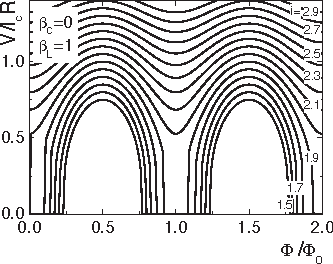
\includegraphics{figures/example_SQI.pdf}
	\caption{Normalized dc-SQUID voltage ($V/I_cR$) over normalized flux ($\Phi_a/\Phi_0$). The lines are for constant current $i=I_b/2I_c$. The two parameters are $\beta_c = 0$ and $1$. The figure has been adapted from~\cite{clarkeSQUIDHandbook2004}.}
	\label{fig:example-SQI}
\end{figure}

\subsection{dc-SQUID magnetometer readout}
By passing a bias current $I_B > 2I_c$ through the dc-SQUID a voltage $V_s$ develops. By measuring this voltage and applying an external field you can determine the SQI. Since the periodicity of the SQI is always $\Phi_0$ this allows you to determine the relation between $V_s$ and $\Phi$. You can see in Figure~\ref{fig:example-SQI} that there are (small) regions where the dc-SQUID's response is linear. In this region we can define a transfer function\cite{rogSQUIDontipMagneticMicroscopy2022}:
\begin{equation}
	H = \left. \frac{\partial V_s}{\partial \Phi} \right|_{I_B}
\end{equation}
In the example figure the most sensitive response is obtained for $I_B = 2i$. After the calibration you can determine the flux through the dc-SQUID by measuring its voltage.

For more information on dc-SQUID magnetometry the reader is referred to~\cite{tinkhamIntroductionSuperconductivity,clarkeSQUIDHandbook2004,schmelzSuperconductingQuantumInterference2017}.